\documentclass[tikz,border=3mm]{standalone}
\usepackage[utf8]{inputenc}
\usepackage[T1]{fontenc}
\usepackage{helvet}
\renewcommand{\familydefault}{\sfdefault}
\usetikzlibrary{arrows.meta,positioning}
\begin{document}

\tikzset{every node/.append style={font=\sffamily\small}}
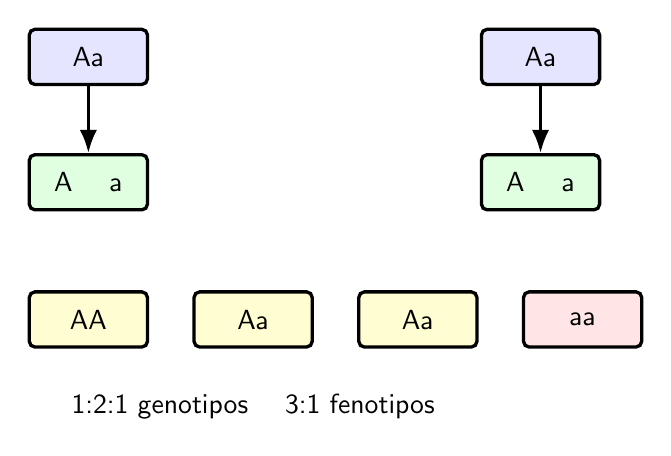
\begin{tikzpicture}[>=Latex,node distance=0.75cm]
  \tikzstyle{box}=[draw,rounded corners=2pt,very thick,align=center,minimum width=1.5cm,minimum height=0.7cm]
  \node[box,fill=blue!10] (p1) {Aa};
  \node[box,fill=blue!10,right=4.2cm of p1] (p2) {Aa};
  \node[box,fill=green!12,below=0.85cm of p1] (g1) {A \quad a};
  \node[box,fill=green!12,below=0.85cm of p2] (g2) {A \quad a};
  \draw[very thick,->] (p1) -- (g1);
  \draw[very thick,->] (p2) -- (g2);
  \node[box,fill=yellow!18,below=1.0cm of g1] (AA) {AA};
  \node[box,fill=yellow!18,right=0.55cm of AA] (Aa1) {Aa};
  \node[box,fill=yellow!18,right=0.55cm of Aa1] (Aa2) {Aa};
  \node[box,fill=red!10,right=0.55cm of Aa2] (aa) {aa};
  \node[align=center,below=0.45cm of Aa1] {1:2:1 genotipos \quad 3:1 fenotipos};
\end{tikzpicture}
\end{document}
